% Options for packages loaded elsewhere
\PassOptionsToPackage{unicode}{hyperref}
\PassOptionsToPackage{hyphens}{url}
%
\documentclass[
]{article}
\usepackage{amsmath,amssymb}
\usepackage{lmodern}
\usepackage{iftex}
\ifPDFTeX
  \usepackage[T1]{fontenc}
  \usepackage[utf8]{inputenc}
  \usepackage{textcomp} % provide euro and other symbols
\else % if luatex or xetex
  \usepackage{unicode-math}
  \defaultfontfeatures{Scale=MatchLowercase}
  \defaultfontfeatures[\rmfamily]{Ligatures=TeX,Scale=1}
\fi
% Use upquote if available, for straight quotes in verbatim environments
\IfFileExists{upquote.sty}{\usepackage{upquote}}{}
\IfFileExists{microtype.sty}{% use microtype if available
  \usepackage[]{microtype}
  \UseMicrotypeSet[protrusion]{basicmath} % disable protrusion for tt fonts
}{}
\makeatletter
\@ifundefined{KOMAClassName}{% if non-KOMA class
  \IfFileExists{parskip.sty}{%
    \usepackage{parskip}
  }{% else
    \setlength{\parindent}{0pt}
    \setlength{\parskip}{6pt plus 2pt minus 1pt}}
}{% if KOMA class
  \KOMAoptions{parskip=half}}
\makeatother
\usepackage{xcolor}
\IfFileExists{xurl.sty}{\usepackage{xurl}}{} % add URL line breaks if available
\IfFileExists{bookmark.sty}{\usepackage{bookmark}}{\usepackage{hyperref}}
\hypersetup{
  hidelinks,
  pdfcreator={LaTeX via pandoc}}
\urlstyle{same} % disable monospaced font for URLs
\usepackage[margin=1in]{geometry}
\usepackage{graphicx}
\makeatletter
\def\maxwidth{\ifdim\Gin@nat@width>\linewidth\linewidth\else\Gin@nat@width\fi}
\def\maxheight{\ifdim\Gin@nat@height>\textheight\textheight\else\Gin@nat@height\fi}
\makeatother
% Scale images if necessary, so that they will not overflow the page
% margins by default, and it is still possible to overwrite the defaults
% using explicit options in \includegraphics[width, height, ...]{}
\setkeys{Gin}{width=\maxwidth,height=\maxheight,keepaspectratio}
% Set default figure placement to htbp
\makeatletter
\def\fps@figure{htbp}
\makeatother
\setlength{\emergencystretch}{3em} % prevent overfull lines
\providecommand{\tightlist}{%
  \setlength{\itemsep}{0pt}\setlength{\parskip}{0pt}}
\setcounter{secnumdepth}{-\maxdimen} % remove section numbering
\ifLuaTeX
  \usepackage{selnolig}  % disable illegal ligatures
\fi

\author{}
\date{\vspace{-2.5em}}

\begin{document}

\hypertarget{oce}{%
\section{\texorpdfstring{oce }{oce }}\label{oce}}

\href{https://joss.theoj.org/papers/10.21105/joss.03594}{\includegraphics{https://joss.theoj.org/papers/10.21105/joss.03594/status.svg}}
\href{https://github.com/dankelley/oce/actions}{\includegraphics{https://github.com/dankelley/oce/workflows/R-CMD-check/badge.svg}}
\href{https://app.codecov.io/gh/dankelley/oce?branch=develop}{\includegraphics{https://codecov.io/gh/dankelley/oce/branch/develop/graph/badge.svg}}
\href{https://cran.r-project.org/package=oce}{\includegraphics{https://www.r-pkg.org/badges/version/oce}}
\includegraphics{https://cranlogs.r-pkg.org/badges/last-month/oce}
\includegraphics{https://cranlogs.r-pkg.org/badges/last-week/oce}
\includegraphics{https://cranlogs.r-pkg.org/badges/last-day/oce}

\hypertarget{why-use-r-for-oceanographic-analysis}{%
\subsection{Why use R for oceanographic
analysis?}\label{why-use-r-for-oceanographic-analysis}}

The R language is popular in many branches of science, and Oceanography
is no exception. With its broad statistical support, R is a natural
choice for oceanographers in the biological, chemical and geological
sub-disciplines. However, some physical oceanographers have remained
attached to Matlab, which was widely adopted during the 1990s. Lately,
this has been changing, as oceanographers turn to open-source systems
such as Python and R. A particular strength of R is its provision of
many powerful and well-vetted packages for handling specialized
calculations. The oce package is a prime example.

\hypertarget{about-oce}{%
\subsection{About oce}\label{about-oce}}

The oce package handles a wide variety of tasks that come up in the
analysis of Oceanographic data. In addition to the present README file,
a brief sketch of the package has been written by the core developers
(Kelley Dan E., Clark Richards and Chantelle Layton, 2022.
\href{https://doi.org/10.21105/joss.03594}{oce: an R package for
Oceanographic Analysis}. Journal of Open Source Software, 7(71), 3594),
and the primary developer uses the package extensively in his book about
the place of R in oceanographic analysis (Kelley, Dan E., 2018.
\href{https://link.springer.com/us/book/9781493988426}{Oceanographic
Analysis with R}. New York. Springer-Verlag ISBN 978-1-4939-8844-0).
Details of oce functions are provided within the R help system, and in
the package \href{https://dankelley.github.io/oce/}{webpage}.

\hypertarget{installing-oce}{%
\subsection{Installing oce}\label{installing-oce}}

Stable versions of oce are available from CRAN, and may be installed
from within R, in the same way as other packages. However, the CRAN
version is only updated a few times a year (pursuant to policy), so many
users install the \texttt{"develop"} branch instead. This branch may be
updated several times per day, as the authors fix bugs or add features
that are motivated by day-to-day usage. This is the branch favoured by
users who need new features or who would wish to contribute to Oce
development.

The easy way to install the \texttt{"develop"} branch is to execute the
following commands in R.

\begin{verbatim}
remotes::install_github("dankelley/oce", ref="develop")
\end{verbatim}

and most readers should also install Ocedata, with

\begin{verbatim}
remotes::install_github("dankelley/ocedata", ref="main")
\end{verbatim}

\hypertarget{evolution-of-oce}{%
\subsection{Evolution of oce}\label{evolution-of-oce}}

Oce is emphatically an open-source system, and so the participation of
users is very important. This is why Git is used for version control of
the Oce source code, and why GitHub is the host for that code. Users are
invited to take part in the development process, by suggesting features,
by reporting bugs, or just by watching as others do such things.
Oceanography is a collaborative discipline, so it makes sense that the
evolution of Oce be similarly collaborative.

\hypertarget{examples-using-built-in-datasets}{%
\subsection{Examples using built-in
datasets}\label{examples-using-built-in-datasets}}

\hypertarget{ctd}{%
\subsubsection{CTD}\label{ctd}}

\begin{verbatim}
library(oce)
data(ctd)
plot(ctd, which=c(1,2,3,5), type="l", span=150)
\end{verbatim}

\begin{figure}
\centering
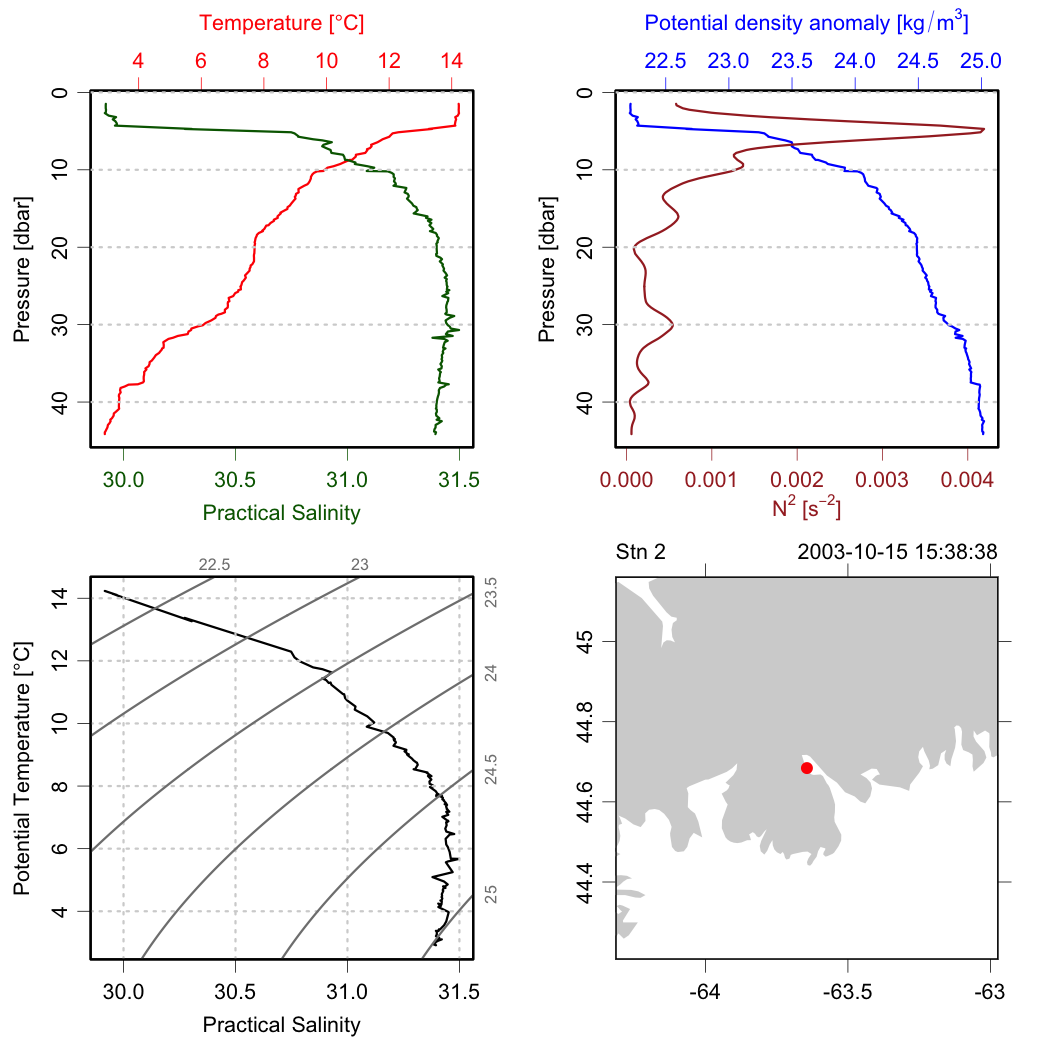
\includegraphics{https://raw.githubusercontent.com/dankelley/oce/develop/oce-demo-1.png}
\caption{Sample CTD plot.}
\end{figure}

\hypertarget{acoustic-doppler-profiler}{%
\subsubsection{Acoustic Doppler
profiler}\label{acoustic-doppler-profiler}}

\begin{verbatim}
library(oce)
data(adp)
plot(adp)
\end{verbatim}

\begin{figure}
\centering
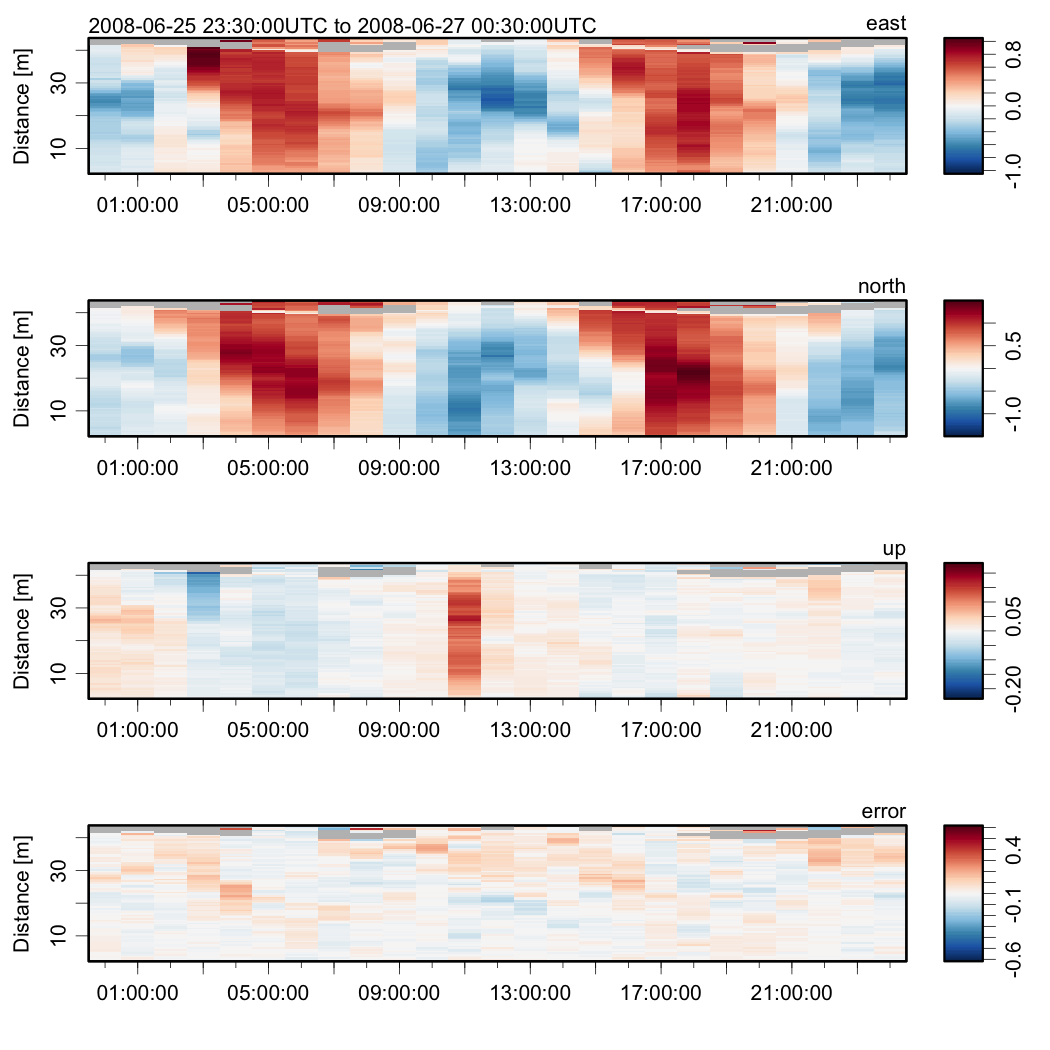
\includegraphics{https://raw.githubusercontent.com/dankelley/oce/develop/oce-demo-2.png}
\caption{Sample adp plot.}
\end{figure}

\hypertarget{sealevel-and-tides}{%
\subsubsection{Sealevel and tides}\label{sealevel-and-tides}}

\begin{verbatim}
library(oce)
data(sealevel)
m <- tidem(sealevel)
par(mfrow=c(2, 1))
plot(sealevel, which=1)
plot(m)
\end{verbatim}

\begin{figure}
\centering
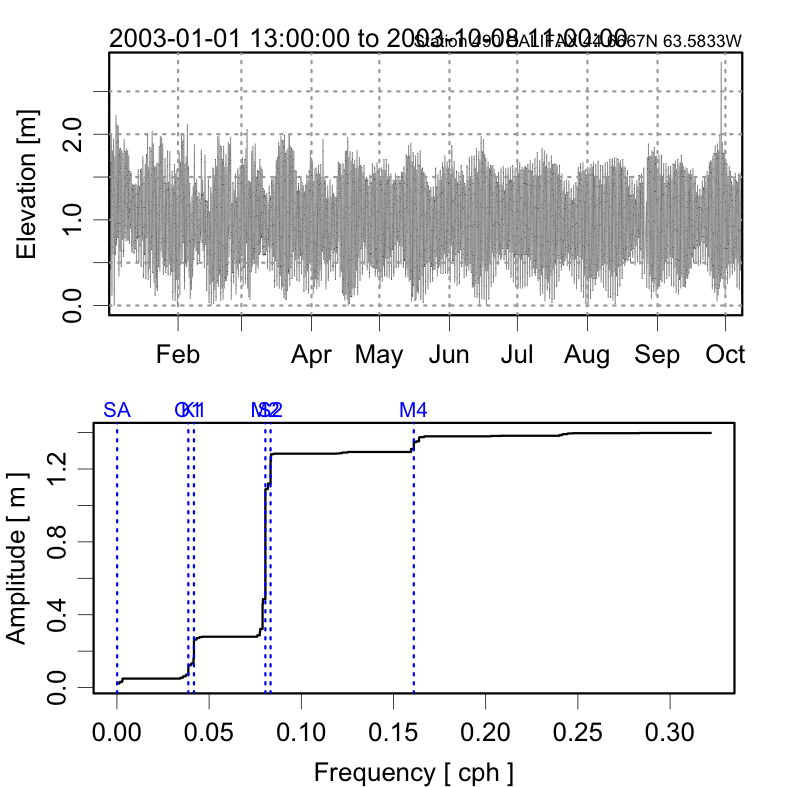
\includegraphics{https://raw.githubusercontent.com/dankelley/oce/develop/oce-demo-3.png}
\caption{Sample sealevel plot.}
\end{figure}

\hypertarget{echosounder}{%
\subsubsection{Echosounder}\label{echosounder}}

\begin{verbatim}
library(oce)
data(echosounder)
plot(echosounder, which=2, drawTimeRange=TRUE, drawBottom=TRUE)
\end{verbatim}

\begin{figure}
\centering
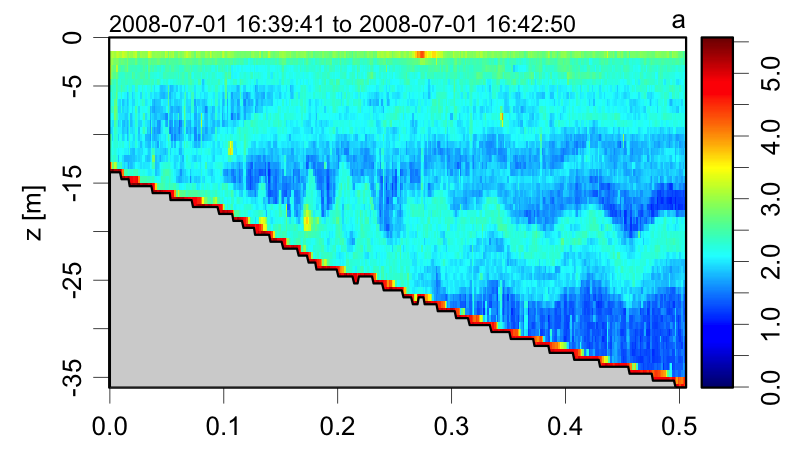
\includegraphics{https://raw.githubusercontent.com/dankelley/oce/develop/oce-demo-4.png}
\caption{Sample echosounder plot.}
\end{figure}

\hypertarget{map}{%
\subsubsection{Map}\label{map}}

\begin{verbatim}
library(oce)
par(mar=rep(0.5, 4))
data(endeavour, package="ocedata")
data(coastlineWorld, package="oce")
mapPlot(coastlineWorld, col="gray")
mapPoints(endeavour$longitude, endeavour$latitude, pch=20, col="red")
\end{verbatim}

\begin{figure}
\centering
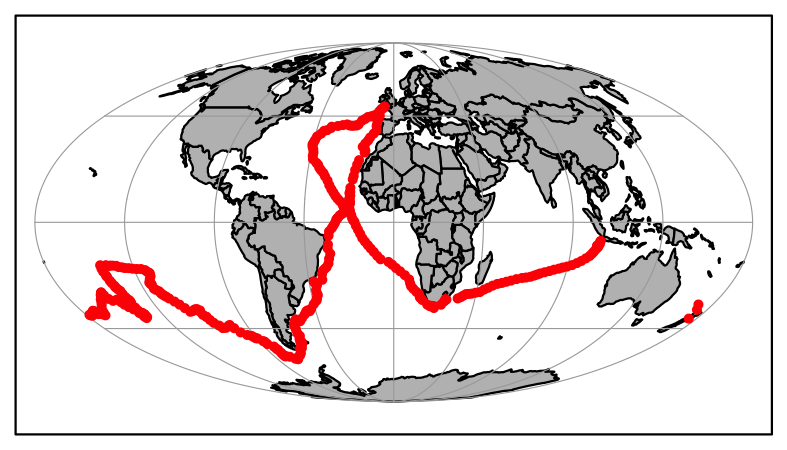
\includegraphics{https://raw.githubusercontent.com/dankelley/oce/develop/oce-demo-5.png}
\caption{Sample map plot.}
\end{figure}

\hypertarget{landsat-image}{%
\subsubsection{Landsat image}\label{landsat-image}}

\begin{verbatim}
library(ocedata)
library(oce)
data(landsat)
plot(landsat)
\end{verbatim}

\begin{figure}
\centering
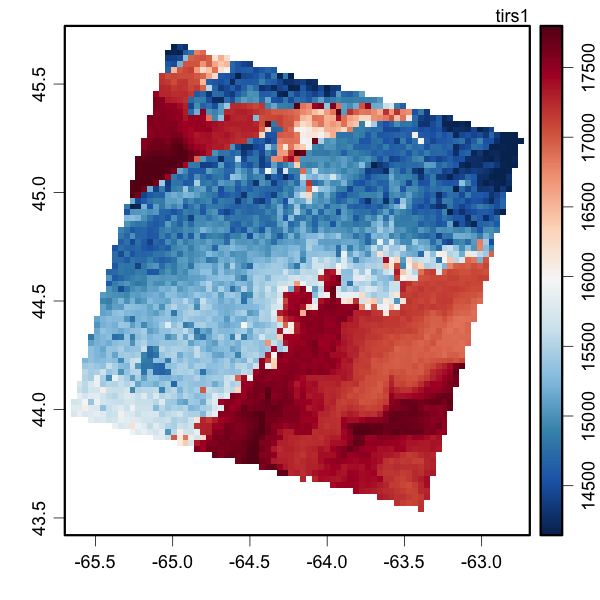
\includegraphics{https://raw.githubusercontent.com/dankelley/oce/develop/oce-demo-6.png}
\caption{Sample landsat image plot.}
\end{figure}

\end{document}
